%%% Article: Software System for Data Acquisition and Analysis Operating the ATLAS-TPX Network
%%% Authors: Petr Manek, Jakub Begera
%%% Copyright (c) 2017 IEAP CTU


% Document Class Definition
\documentclass[conference,a4paper]{IEEEtran}
\usepackage[a4paper]{geometry}
\geometry{top=20mm, bottom=20mm, left=30mm, right=20mm, twoside=true}


% Package Dependencies
\usepackage{color}
\usepackage{isotope}
\usepackage{graphicx,subfigure}
\usepackage{dcolumn}
\usepackage{bm}
\usepackage[utf8]{inputenc}
\usepackage[pdfborder=000,pdftex=true,bookmarks=false]{hyperref}
\usepackage{amsmath}
\usepackage{balance}
\usepackage{flushend}


% Document Content Begins Here
\begin{document}


% Header
\title{Software System for Data Acquisition and Analysis Operating the ATLAS-TPX Network}

\author{\IEEEauthorblockN{
Petr~Manek$^{*}$,
Jakub~Begera$^{*}$,
Benedikt~Bergmann$^{*}$,
Petr~Burian$^{*,\dagger}$,
Josef~Janecek$^{*}$,\\
Stepan~Polansky$^{*}$,
Stanislav~Pospisil$^{*}$ and
Michal~Suk$^{*}$}
\IEEEauthorblockA{$^{*}$Institute of Experimental and Applied Physics\\
Czech Technical University in Prague,
Horska 3a/22, 128 00 Praha 2-Albertov, Czech Republic\\ Email: petr.manek@cvut.cz, jakub.begera@cvut.cz}
\IEEEauthorblockA{$^{\dagger}$Faculty of Electrical Engineering\\
University of West Bohemia, Univerzitni 26, 306 14 Plzen, Czech Republic}}

\markboth{}%
{P. Manek, J. Begera \MakeLowercase{\textit{et al.}}: Software System for Data Acquisition and Analysis Operating the ATLAS-TPX Network}

\maketitle


% 2-Column Content
\begin{abstract}
A network of 15 Timepix pixel detectors was installed within the ATLAS experiment at CERN, Geneva. The network is capable of measuring the composition and spectral characteristics of the radiation fields in real-time. Its operation is managed by a dedicated software system. The presented article describes primary software components of this system responsible for communication with detector hardware, online operation monitoring, remote acquisition control, automated data verification and analysis. The processed data can be accessed through an interactive web-based Data Visualization Application, which is available to the scientific community.
\end{abstract}

%%% Article: Software System for Data Acquisition and Analysis Operating the ATLAS-TPX Network
%%% Authors: Petr Manek, Jakub Begera
%%% Copyright (c) 2017 IEAP CTU


\section{\label{sec:introduction}Introduction}
The ATLAS-MPX Network has been installed in the ATLAS cavern at the LHC at CERN~\cite{CampbellATLAS}. During the 2013-2014 shut-down period this network was upgraded to a two-layer Timepix design (ATLAS-TPX) with a faster readout system and improved capabilities to discriminate charged particles and gamma rays against neutrons~\cite{Proposal_Claude,Bergmann_ATLASTPX_2016}.

Operation of the network is managed by a distributed software system comprised of several independent components:
~
\begin{itemize}
  \item The Acquisition and Control Subsystem handles communication with detectors through the readout interface.
  \item The Data Analysis Subsystem automatically verifies and processes frames taken by detectors.
  \item The Data Visualization Application displays processed data in the form of pixel matrices and trace flux charts.
\end{itemize}

%%% Article: Software System for Data Acquisition and Analysis Operating the ATLAS-TPX Network
%%% Authors: Petr Manek, Jakub Begera
%%% Copyright (c) 2017 IEAP CTU


\section{\label{sec:device}Device Design}
Each ATLAS-TPX device consists of two Timepix~\cite{Llopart2007} readout chips with silicon sensor layers of thicknesses 300\,$\mu$m and 500\,$\mu$m facing each other~\cite{Bergmann_ATLASTPX_2016}. They are interlaced by a set of neutron converters. The Timepix ASIC (application specific integrated circuit) divides the sensor area into a square matrix of $256 \times 256$ contiguous pixels with a pixel dimension of 55\,$\mu$m. It allows a configuration of each pixel in either of the three modes of operation: 
~
\begin{itemize}
  \item In the spectroscopic Time-over-Threshold (ToT) mode the energy deposition in the sensor material is measured.
  \item In the Time-of-Arrival (ToA) mode the time from an interaction with respect to the end of the exposure is recorded (precision up to 25\,ns).
  \item In the counting mode, the number of interactions with energies above 5\,keV during the exposure time are counted.
\end{itemize}

Data are taken in so-called frames, representing the counter contents of all individual pixels after an adjustable exposure time (often also referred to as frame acquisition time). In each frame, interacting quanta of ionizing radiation can be seen as tracks on the pixel matrix, which have characteristic shapes, depending on the particle range in silicon, its deposited energy, angle of incidence, and particle type~\cite{Holy2008}.


%%% Article: Software System for Data Acquisition and Analysis Operating the ATLAS-TPX Network
%%% Authors: Petr Manek, Jakub Begera
%%% Copyright (c) 2017 IEAP CTU


\section{\label{sec:hardware}Hardware Architecture}
Given the harsh radiation environment within the ATLAS machine, ATLAS-TPX devices have to be connected to the rest of the system through a dedicated readout interface. This readout is a special hardware device that reads data and controls acquisition of the detector. The ATLASPIX readout (see Fig.~\ref{fig:device_with_readout}) was developed by modifying a regular FITPix readout~\cite{FITPix}.

\begin{figure}[tbp]
	\centering
  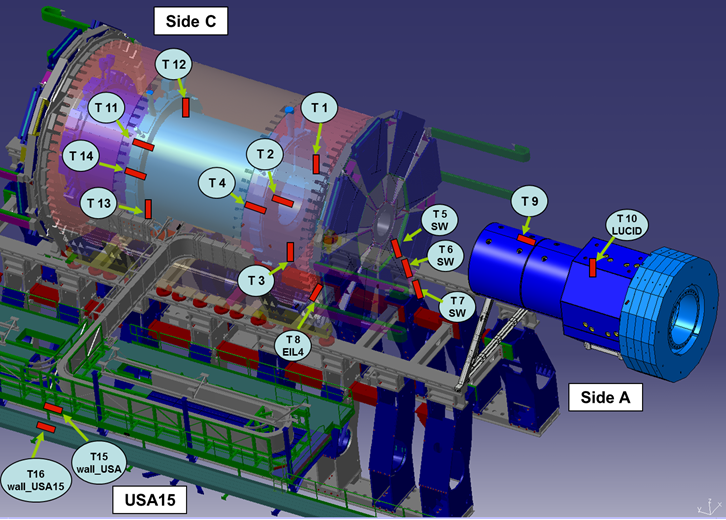
\includegraphics[clip, width=.45\textwidth, angle=0]{Plots/ATLASTPX.png}
  \caption {Artistic view of the device positions of the ATLAS-TPX network in the ATLAS experiment.}
  \label{fig:positions}
\end{figure}

The readout has two parts connected by four cables. The detector itself is positioned and oriented within the ATLAS machine (see Fig.~\ref{fig:positions}), whereas the rest of the readout is placed in a nearby server room, shielded against ionizing radiation. Cables connect both parts, allowing protected hardware to control detectors remotely during operation of the machine. To manage multiple detectors simultaneously, a computer is directly connected to all readouts. This \textit{Control PC} gathers all measured data and forwards commands from the system operator to the detectors through the ATLASPIX readout.

\begin{figure}[tbp]
	\centering
  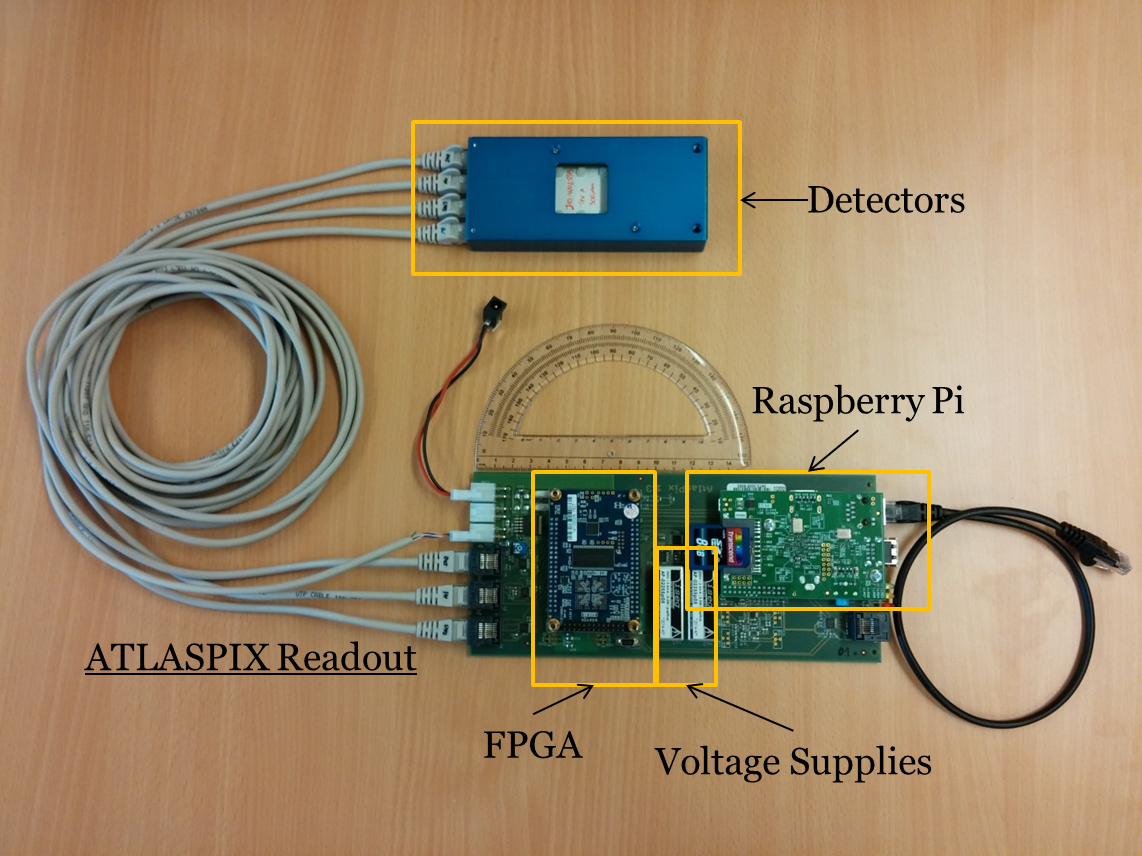
\includegraphics[clip, width=.45\textwidth, angle=0]{Plots/ATLASPIX.png}
  \caption {ATLAS-TPX device, connected to its readout system through three Ethernet cables. The readout system consists of an FPGA, handling the device settings and operation, and a Raspberry Pi minicomputer for sending the data to the control PC in human readable format. Two voltage supplies are used for feeding the proper bias to each of the sensor layers.}
  \label{fig:device_with_readout}
\end{figure}

The Control PC (seen in Fig.~\ref{fig:rack}) is connected directly to the ATLAS Technical Network, which is isolated from the rest of CERN network infrastructure. Consequently, all communications outside the network have to utilize other systems. Acquisition control and real-time status monitoring of the network uses DCS (Detector Control System). Measured data are transferred to the EOS distributed storage system~\cite{MAscetti2015,Peters2011}.

\begin{figure}[tbp]
	\centering
  \includegraphics[clip, width=.33\textwidth, angle=0]{Plots/rack_usa15.pdf}
  \caption {TPX rack in the shielded technical room USA15 in the ATLAS cavern. The photo shows the installed ATLASPIX readouts connected to the Control PC, which communicates with DCS, EOS and FSM over the ATLAS Technical Network.}
  \label{fig:rack}
\end{figure}


%%% Article: Software System for Data Acquisition and Analysis Operating the ATLAS-TPX Network
%%% Authors: Petr Manek, Jakub Begera
%%% Copyright (c) 2017 IEAP CTU


\section{\label{sec:acquisition}Acquisition \& Control Subsystem}
The ATLAS-TPX network operation is controlled by the Acquisition \& Control Subsystem~\cite{Begera2016} hosted at the Control PC. The primary function of this software is to manage the communication with all ATLASPIX readouts using a dedicated low-level protocol consisting of 19 instructions. These instructions fall into 3 general categories:
~
\begin{enumerate}
  \item Acquisition Control Instructions are used to signal the beginning and the end of the data taking period and to retrieve the measured data from the detectors.
  \item Hardware Configuration Instructions read and modify digital-to-analog and analog-to-digital converter values.
  \item Device Status Queries are used to ascertain the general and the acquisition status of the detectors as well as the ATLASPIX readouts.
\end{enumerate}

The software provides a network interface which allows system operators to control detector acquisition by remotely issuing high-level commands. Translated into low-level instructions, these commands are then sent to the ATLASPIX readouts responsible for their execution.

High-level commands can be issued either through the HTTP REST API, accessible from the ATLAS Technical Network, or through the DCS (Detector Control System), accessible from the ATLAS Control Room. Unlike low-level instructions, these commands need to be transmitted only when changes in detector configuration or acquisition are requested.

The network status monitoring is provided by the FSM (Finite State Machine). During regular operation, the control software periodically queries the status of all ATLASPIX readouts as well as the Control PC itself. This information is then forwarded to the DCS, making it available to the FSM and the network operator in the ATLAS Control Room. The FSM is responsible for the determination of the overall status of the network based on the monitored values and raising alarms when failures are detected. The monitored values include:
~
\begin{itemize}
  \item General status information -- connection status of all detectors and their respective ATLASPIX readouts, critical DAC values.
  \item Acquisition mode settings of all detectors.
  \item Control PC information -- available disk space utilization, CPU, memory load and network throughput.
  \item EOS availability -- connection status and latency.
\end{itemize}

Apart from system health indicators and performance meters, the control software also reports back the results of lightweight real-time data analysis for each detector in operation. These results are calculated and aggregated synchronously during the data taking process, and can therefore serve as a continuous feedback for acquisition parameter correction.


%%% Article: Software System for Data Acquisition and Analysis Operating the ATLAS-TPX Network
%%% Authors: Petr Manek, Jakub Begera
%%% Copyright (c) 2017 IEAP CTU


\section{\label{sec:analysis}Data Analysis Subsystem}
The Data Analysis Subsystem is comprised of virtual machines hosted at the CERN Meyrin data center and managed by the OpenStack private cloud. Each machine provides a multitude of \textit{worker nodes} responsible for parallel execution of queued \textit{jobs} -- mutually independent operations that interact with data files, providing:
~
\begin{itemize}
  \item Cluster analysis -- morphological classification, converter region determination~\cite{Holy2008}, optionally integration with energy calibration~\cite{Jakubek2011}.
  \item Storage format conversions -- from ASCII plain text to ROOT~\cite{ROOT} and vice versa.
  \item Data consistency verification.
  \item Frame quality checks -- Monte Carlo sampling, alerts are generated when frames violate pre-defined quality criteria.
  \item File transfers -- gzip compression and subsequent archive transfers between Control PC in USA15, EOS and Prague storage infrastructure.
\end{itemize}

Scheduling and completion of such jobs as well as the heartbeat and load state of worker nodes is continuously tracked by a single centralized \textit{manager node}, which indirectly communicates with all workers through shared PostgreSQL database cluster. The cluster operates independently of all nodes, providing additional level of robustness to the entire system. It is responsible for maintaining a priority queue for scheduled jobs, a job locking mechanism for worker nodes, periodically updated worker node manifest and alert delivery system. The underlying database middleware ensures appropriate caching, replication, data persistency and transaction ordering control.

The primary purpose of the Data Analysis Subsystem is to provide reliable infrastructure for automated data verification and evaluation. For reasons of stability and security, these tasks are performed asynchronously with respect to each other and incoming data transfers. In addition to processing new frames, this approach also allows data files to be reprocessed when novel analysis algorithms are introduced.

\begin{figure}[tbp]
  \centering
  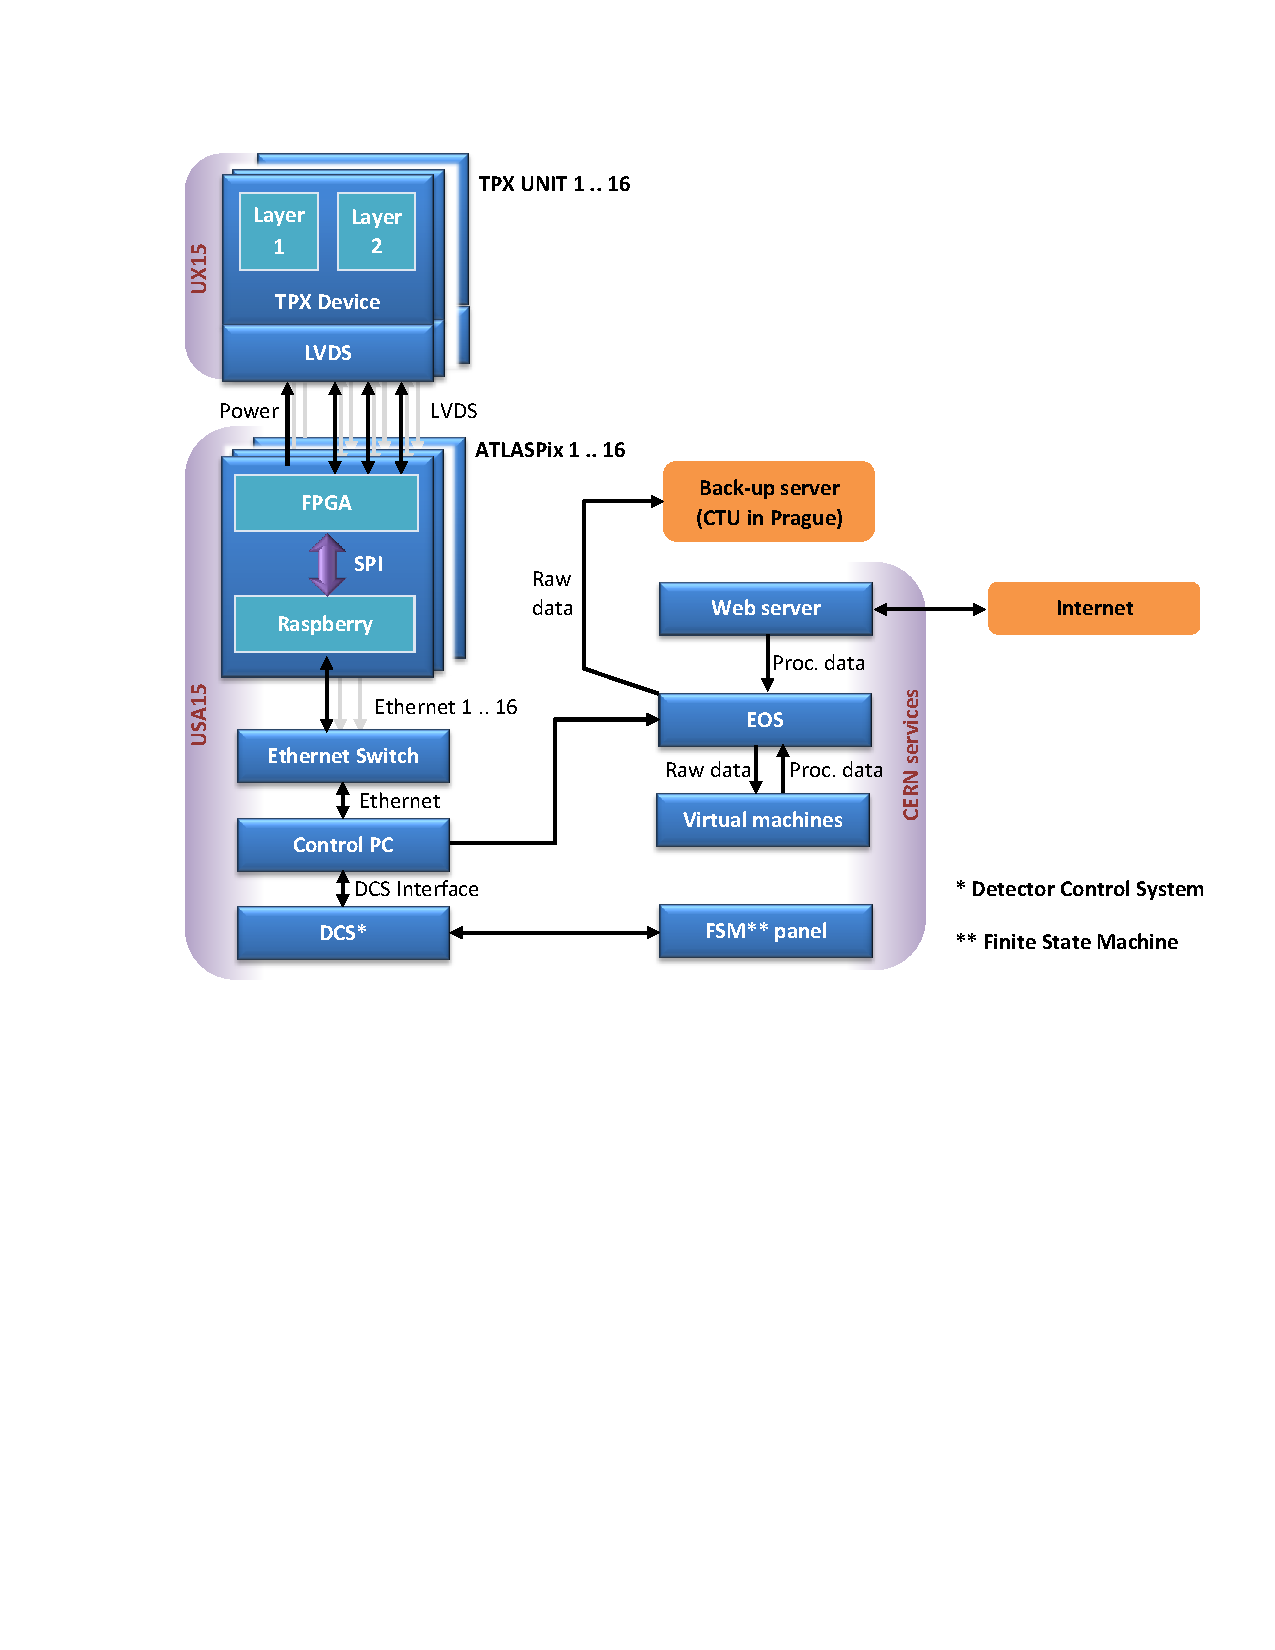
\includegraphics[clip, trim={2cm 11.2cm 0cm 2.6cm}, width=.5\textwidth, angle=0]{Plots/Doc1.pdf}
  \caption{Scheme of the readout, detector control, and data flow.}
  \label{fig:data_flow}
\end{figure}

Usually, frames taken by the TPX detectors are temporarily retained at the Control PC, then transferred to the EOS shared disk pool storage in 1-hour batches (see Fig.~\ref{fig:data_flow}). Once in EOS, data files become available to all users of the system. Due to high redundancy of the ASCII file format, data conversion is performed prior to any subsequent analysis. The conversion process is automatically scheduled as a job by the manager node after the data is confirmed to be valid and no detector malfunctions are suspected. In the course of this operation, frames are subject to cluster analysis~\cite{Holy2008} and measurements are combined with energy calibration data~\cite{Jakubek2011}. Results of this process are stored back in EOS in format compatible with the ROOT Data Analysis Framework~\cite{ROOT}.

The produced files are utilized as a database by the Data Visualization Application. Furthermore, these files serve as a starting point for further analysis performed manually. The original ASCII data files are compressed and downloaded to backup archive media.


%%% Article: Software System for Data Acquisition and Analysis Operating the ATLAS-TPX Network
%%% Authors: Petr Manek, Jakub Begera
%%% Copyright (c) 2017 IEAP CTU


\section{\label{sec:dal}Visualization Application}
Processed data can be examined directly from the ROOT files or by means of the Data Visualization Application. \cite{Manek2016} This application features a web interface capable of displaying frames given specific detector, date and time. In addition, the application is capable of plotting fluxes of characteristic traces in specified time periods. See Fig. \ref{fig:visualizer}.

Since the data is visualized on client-side using modern rendering techniques, the application can also offer basic data operations such as cluster filtering, pixel masking, data aggregation and integral view.

The application serves mainly as a tool of manual inspection of the network operation history. It is openly available to the scientific community upon request.

\begin{figure*}[tbp]
  \centering
  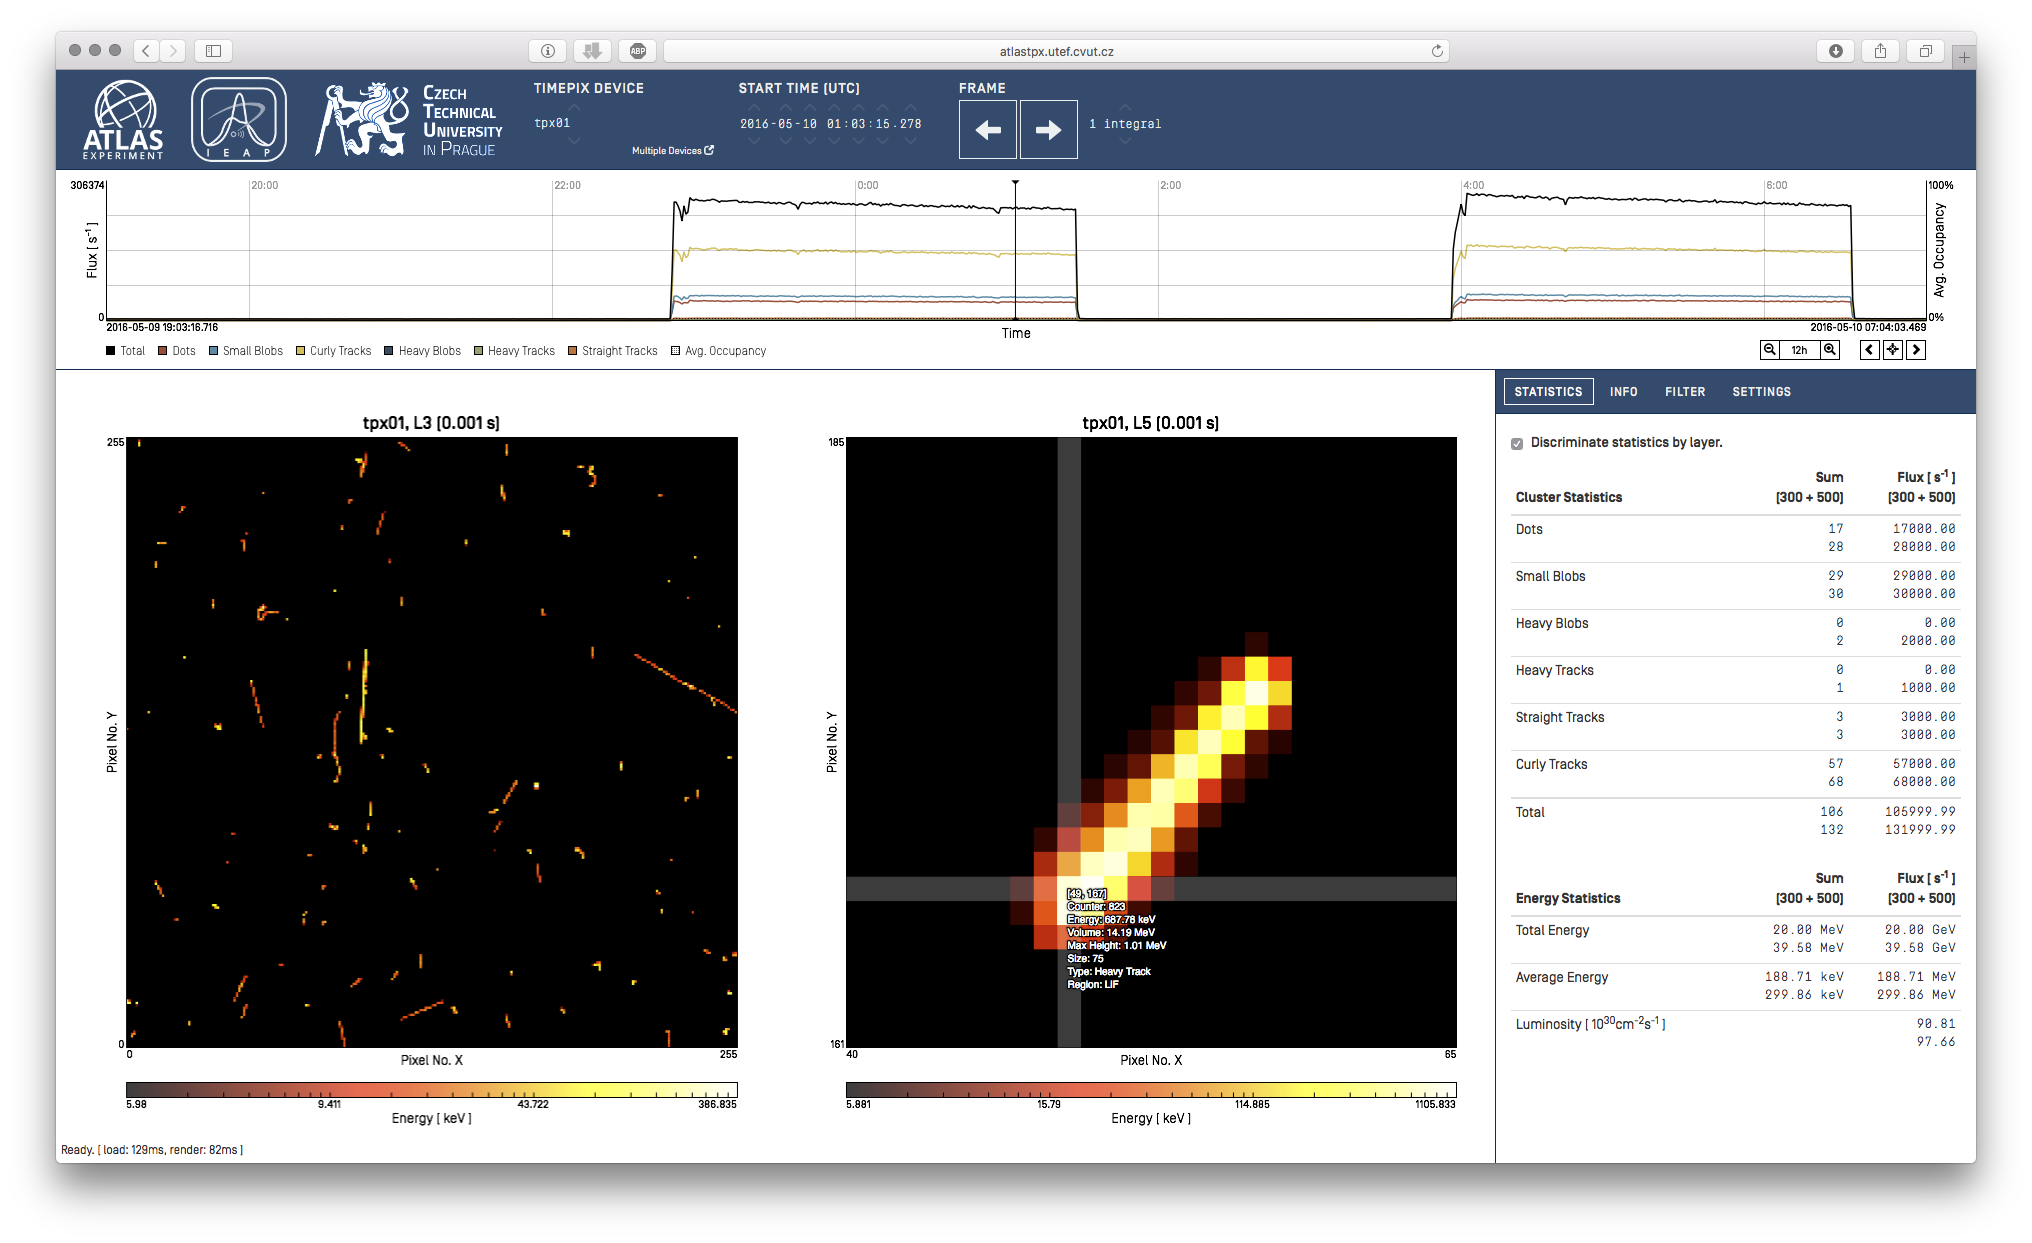
\includegraphics[clip, width=\textwidth, angle = 0 ]{Plots/screen-tpx01-crosshair-zoomed.png}
  \caption {Screenshot of the Data Visualization Application. \cite{Manek2016} Top chart shows occupancy and flux of characteristic traces (differentiated by colors) in frames of specified time range, the vertical line in the middle indicates a selected point in time. Bottom charts show pixel matrices from both TPX sensor layers of a specified detector at the selected time point, the position of the mouse cursor (in the right matrix) is highlighted, showing more information about the trace underneath. Such information includes results of morphological classification, converter region, size, volume, etc. Right sidebar shows a table with characteristic trace counts and fluxes for the displayed frame and interactive filter control interface, which is capable of formulating a custom predicate from cluster and pixel data. The application is available online at \url{https://tpx-visualizer.cern.ch/}, access is granted upon request.}
  \label{fig:visualizer}
\end{figure*}


%%% Article: Software System for Data Acquisition and Analysis Operating the ATLAS-TPX Network
%%% Authors: Petr Manek, Jakub Begera
%%% Copyright (c) 2017 IEAP CTU


\section{\label{sec:conclusion}Conclusion}
A software solution was presented to control acquisition and retrieve, analyze and display frames from the ATLAS-TPX Network. All components of the system are fully operational.

In addition, the presented application has been successfully integrated with TPX detector networks in other CERN experiments such as MoEDAL or ATLAS-GPX. The Data Visualization Application is available to the scientific community upon request.


%%% Article: Software System for Data Acquisition and Analysis Operating the ATLAS-TPX Network
%%% Authors: Petr Manek, Jakub Begera
%%% Copyright (c) 2017 IEAP CTU


\section*{\label{sec:acknowledgements}Acknowledgements}
The work has been done in the frame of the Medipix collaboration. This research project has been supported by the Ministry of Education, Youth and Sports of the Czech Republic under project numbers: LM2015058 and LG15052


\bibliographystyle{IEEEtran}
\bibliography{ieee2016}


\end{document}
